\section[Simplex Algorithm of Nelder and Mead]{Simplex Algorithm of Nelder and Mead with the Extension of O'Neill}
\lab{sec:simAlgNelMea}

The Simplex algorithm of Nelder and Mead is a derivative free optimization algorithm.
It can be used to seek a solution of problem $\mathbf P_c$ defined in~\eqref{sub:Proc} 
and problem $\mathbf P_{cg}$ defined in~\eqref{sub:Procg},
with constraints on the dependent parameters implemented as 
described in Section~\ref{cha:conGen}.
The number of independent parameters $n$ must be larger than 1.\\

The Simplex algorithm constructs an $n$-dimensional simplex
in the space that is spanned by the independent parameters.
At each of the $(n+1)$ vertices of the simplex, the value of the cost function is evaluated. In each iteration step, the point with the highest value of the cost function is replaced by another point. The algorithm consists of three main operations: (a) \emph{point reflection}, (b) \emph{contraction of the simplex} and (c) \emph{expansion of the simplex}.\\


Despite the well known fact 
that the Simplex algorithm can fail to converge to a stationary 
point~\cite{Kelley1999:2,Torczon1989,Kelley1999:1,Wright1996,McKinnon1998,Lagarias1998}, both in practice and theory,
particularly if the dimension of independent variables is large, 
say bigger than $10$~\cite{Torczon1989}, it is an often used algorithm.
Several improvements to the Simplex algorithm
or algorithms that were motivated by the Simplex algorithm exist,
see for example~\cite{Kelley1999:2,Torczon1989,Kelley1999:1,Tseng1999}.
However, in GenOpt, we use the original Nelder-Mead algorithm~\cite{NelderMea1965}
with the extension of O'Neill~\cite{ONeill1971}.
Optionally, the here implemented algorithm allows using
a modified stopping criteria.\\

We will now explain the different steps of the Simplex algorithm.


\subsection{Main Operations}
\begin{figure}
  \centering
  \mbox{ \subfigure[Reflection.]{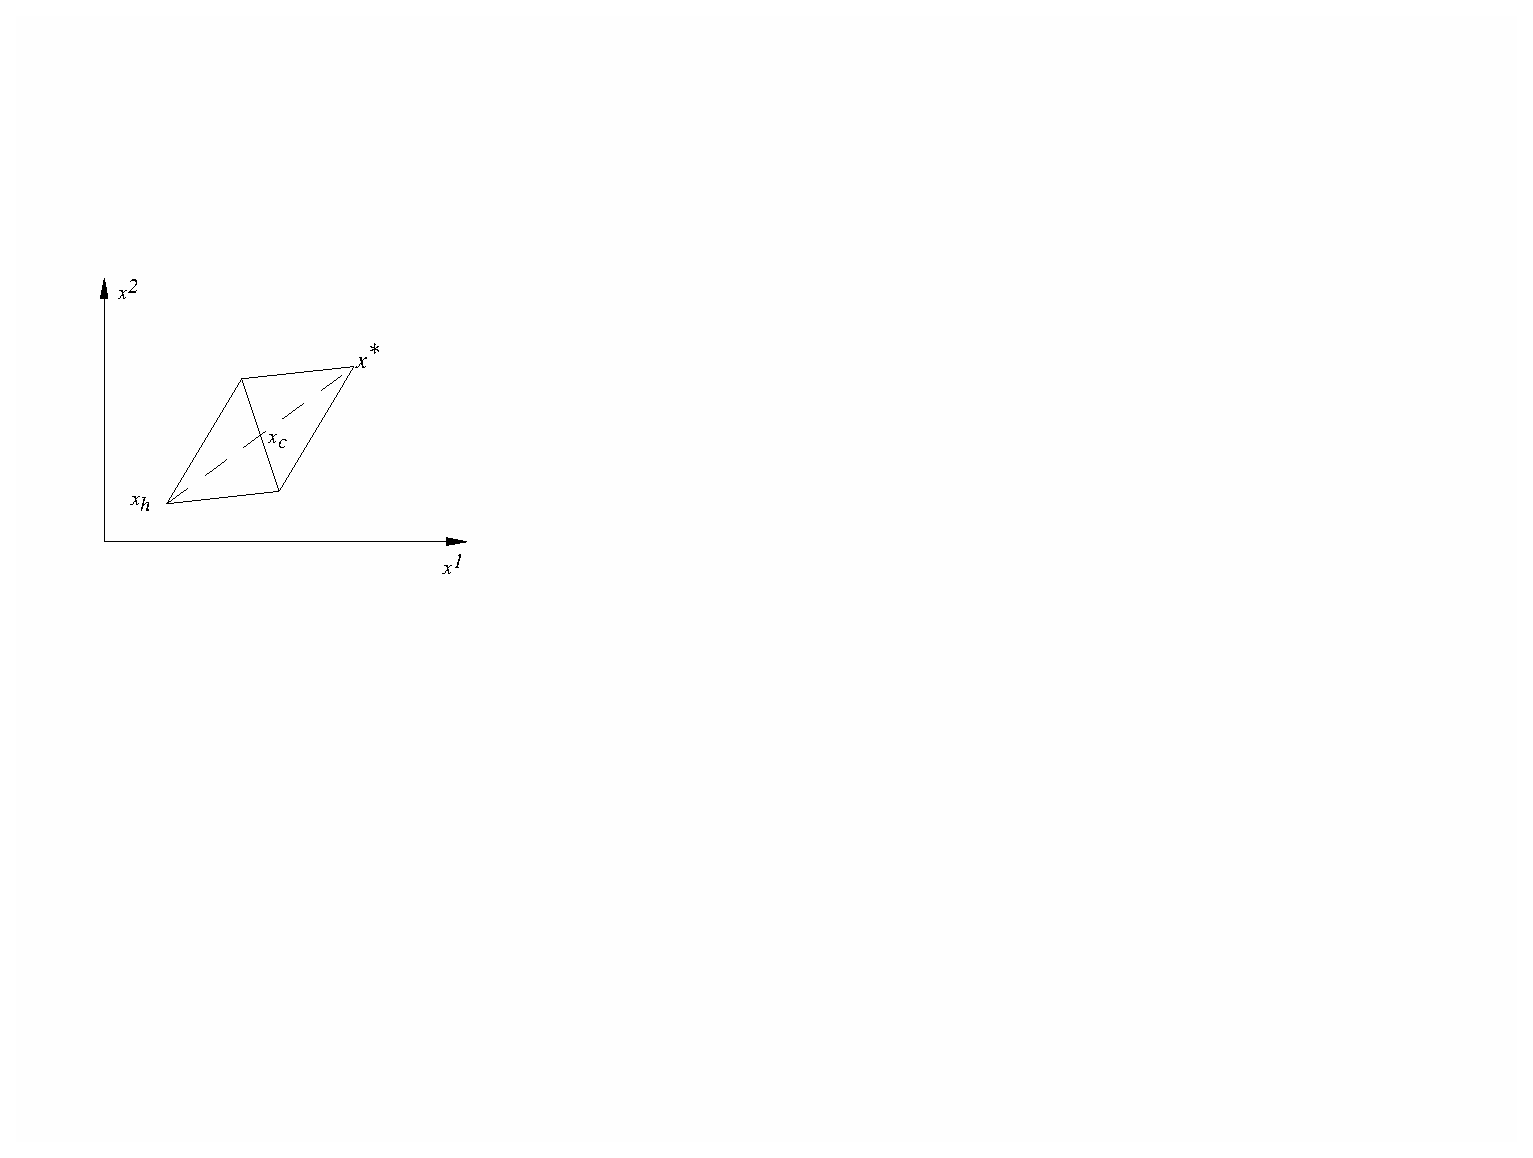
\epsfig
      {file=img/nel_mea_ref.eps, bb=35 265 225 420, scale=0.9, clip=}}
    \subfigure[Expansion.]{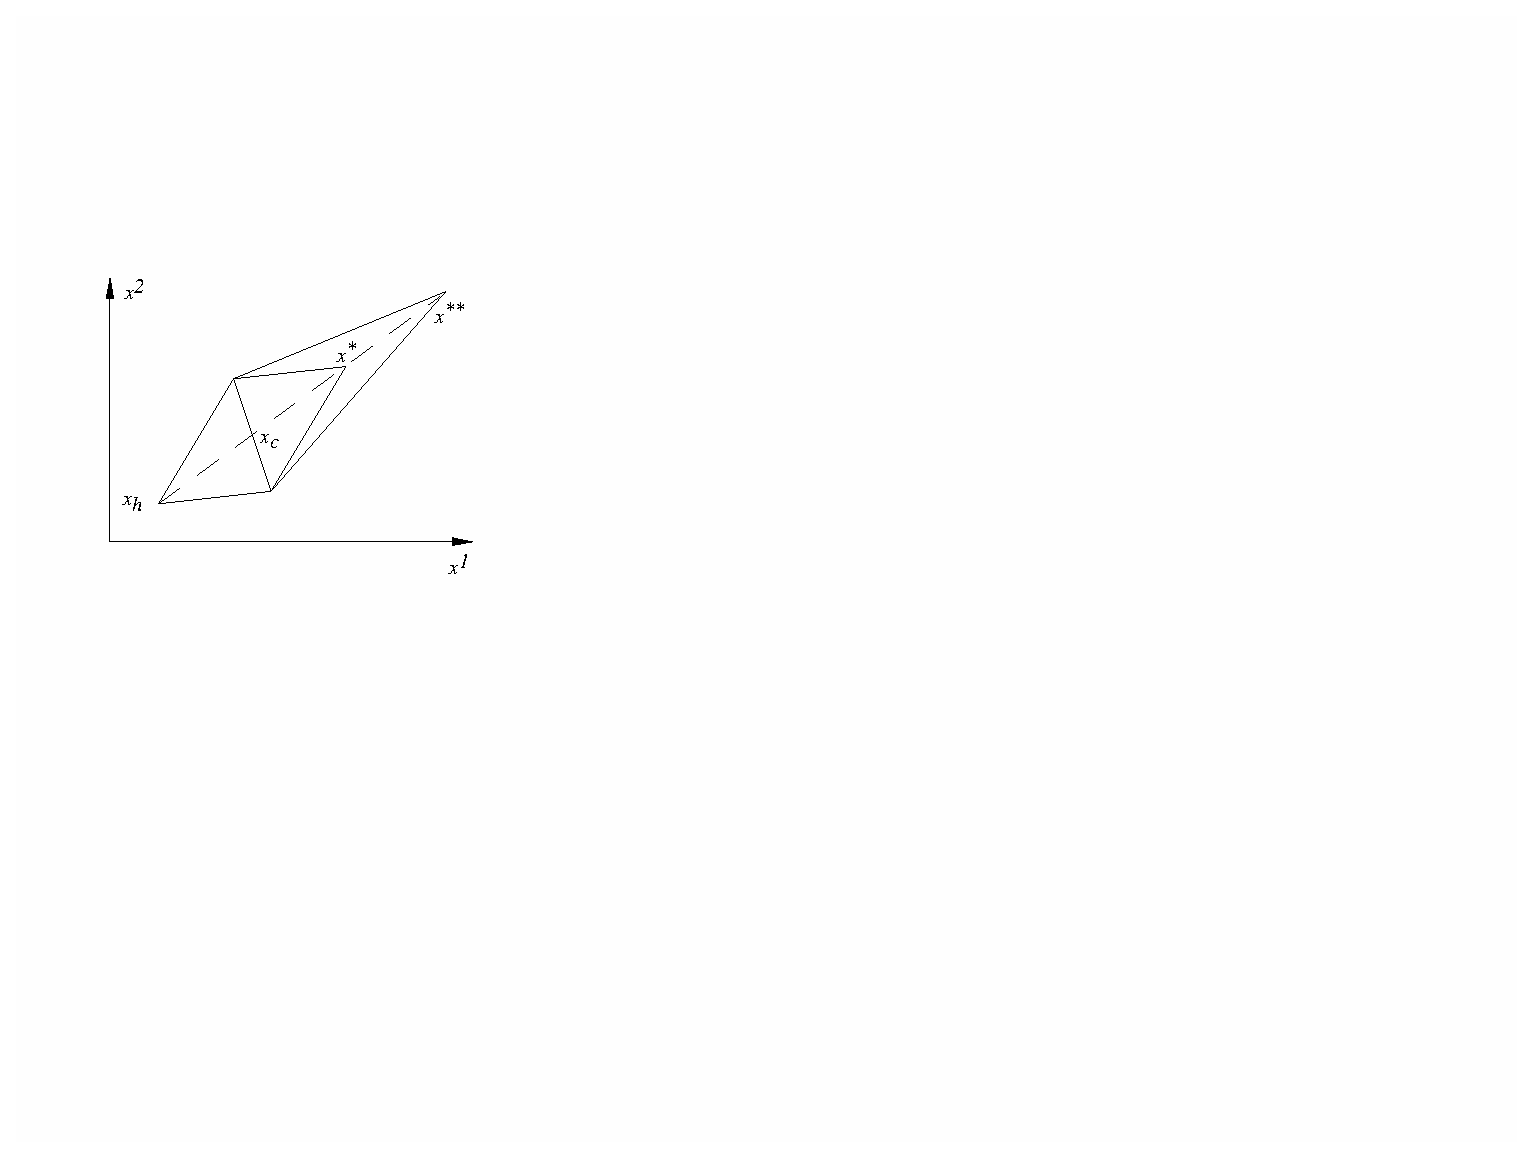
\epsfig
      {file=img/nel_mea_exp.eps, bb=35 265 225 420, scale=0.9, clip=}} }
  \mbox{ 
    \subfigure[Partial inside contraction.]{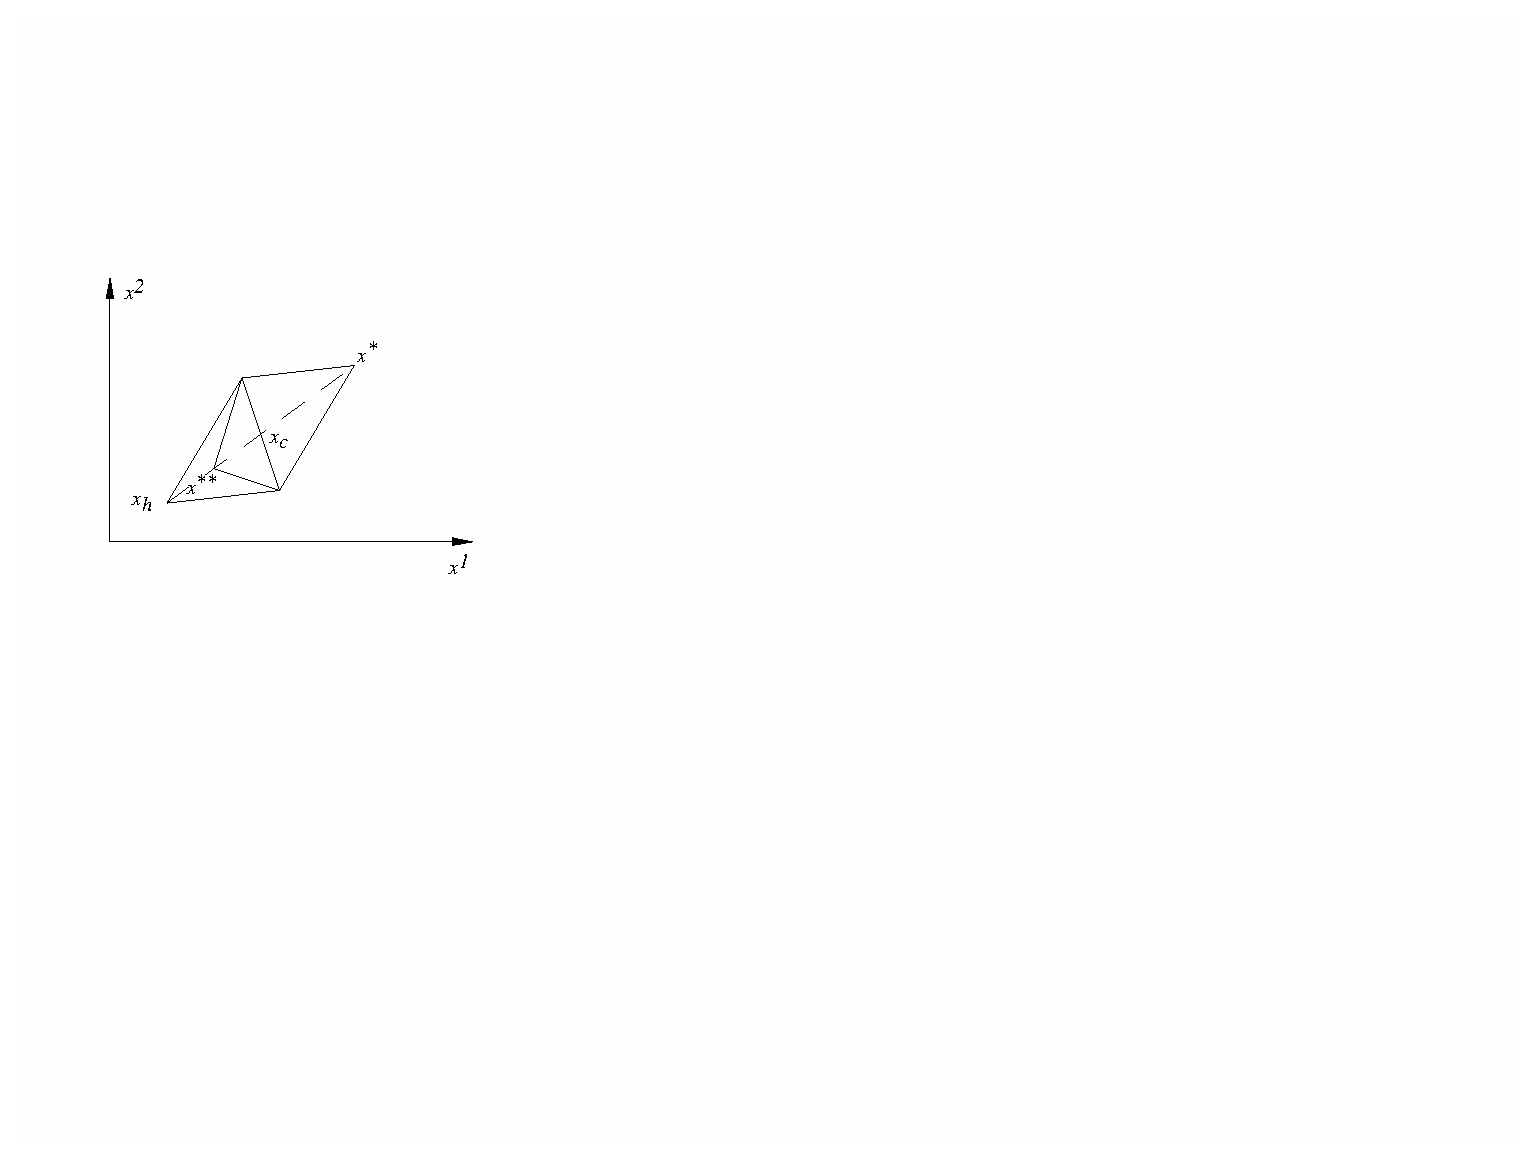
\epsfig
      {file=img/nel_mea_par_ins.eps, bb=35 265 225 420, scale=0.9, clip=}}
    \subfigure[Partial outside contraction.]{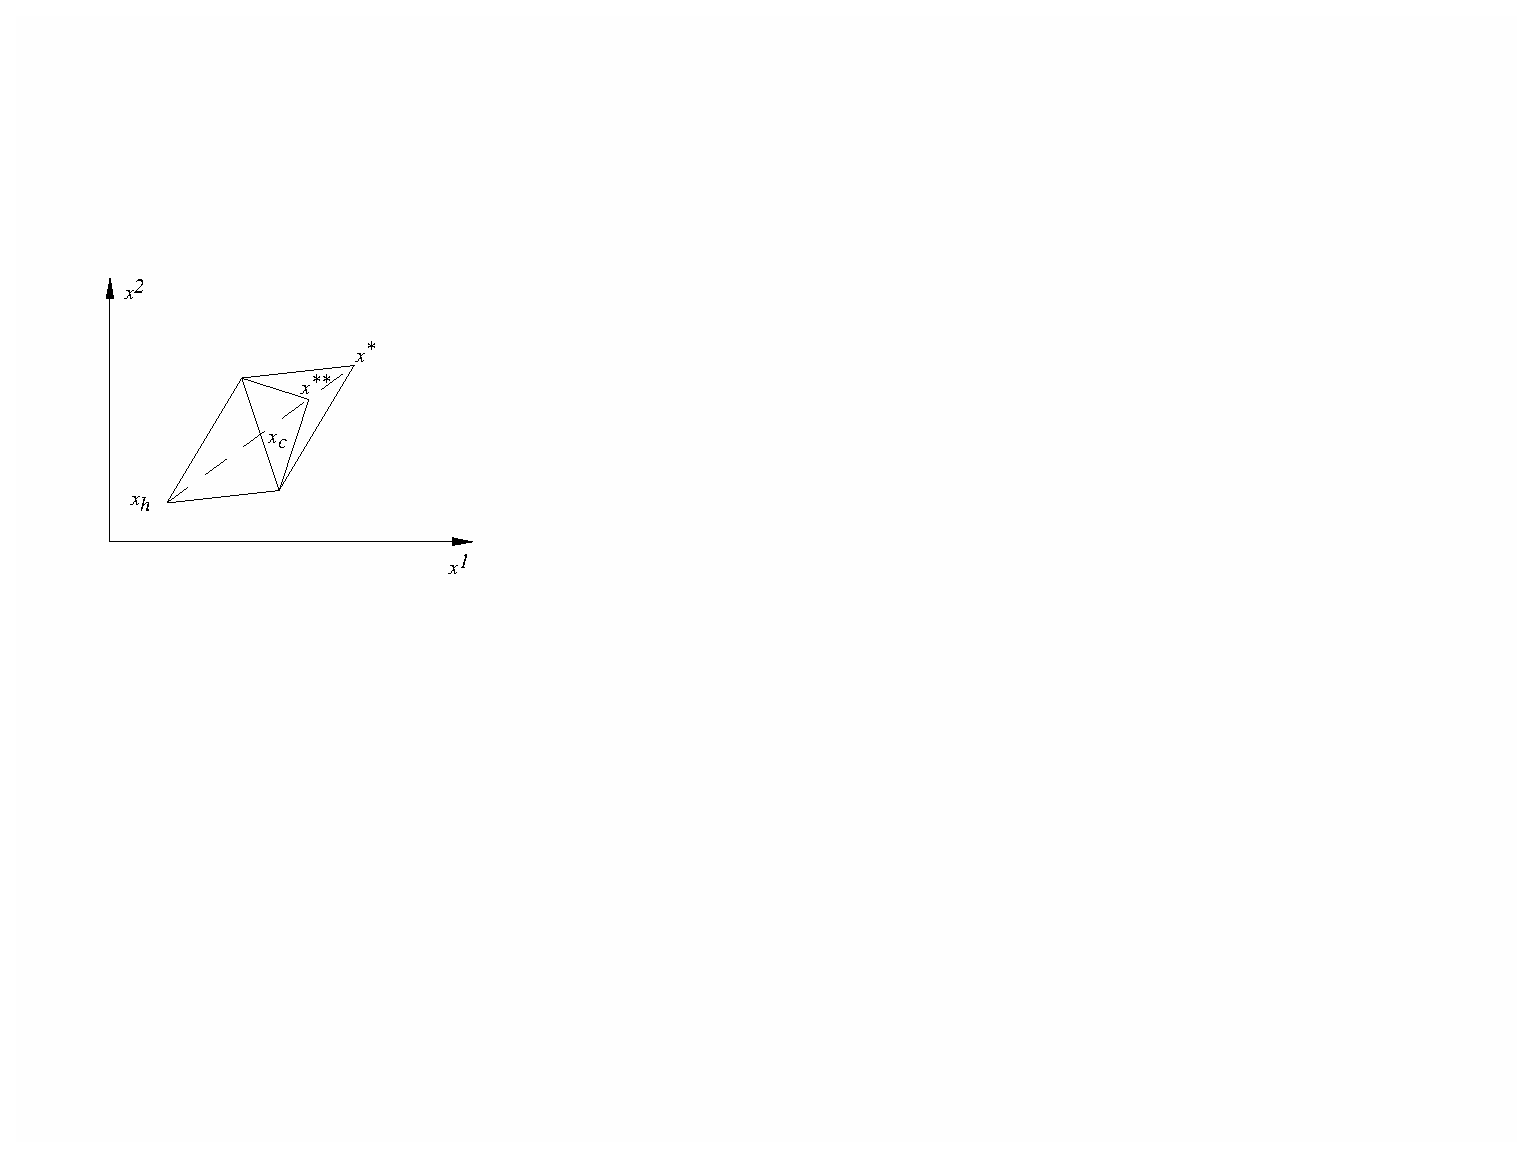
\epsfig
      {file=img/nel_mea_par_out.eps, bb=35 265 225 420, scale=0.9, clip=}} }
  \mbox{
    \subfigure[Total contraction.]{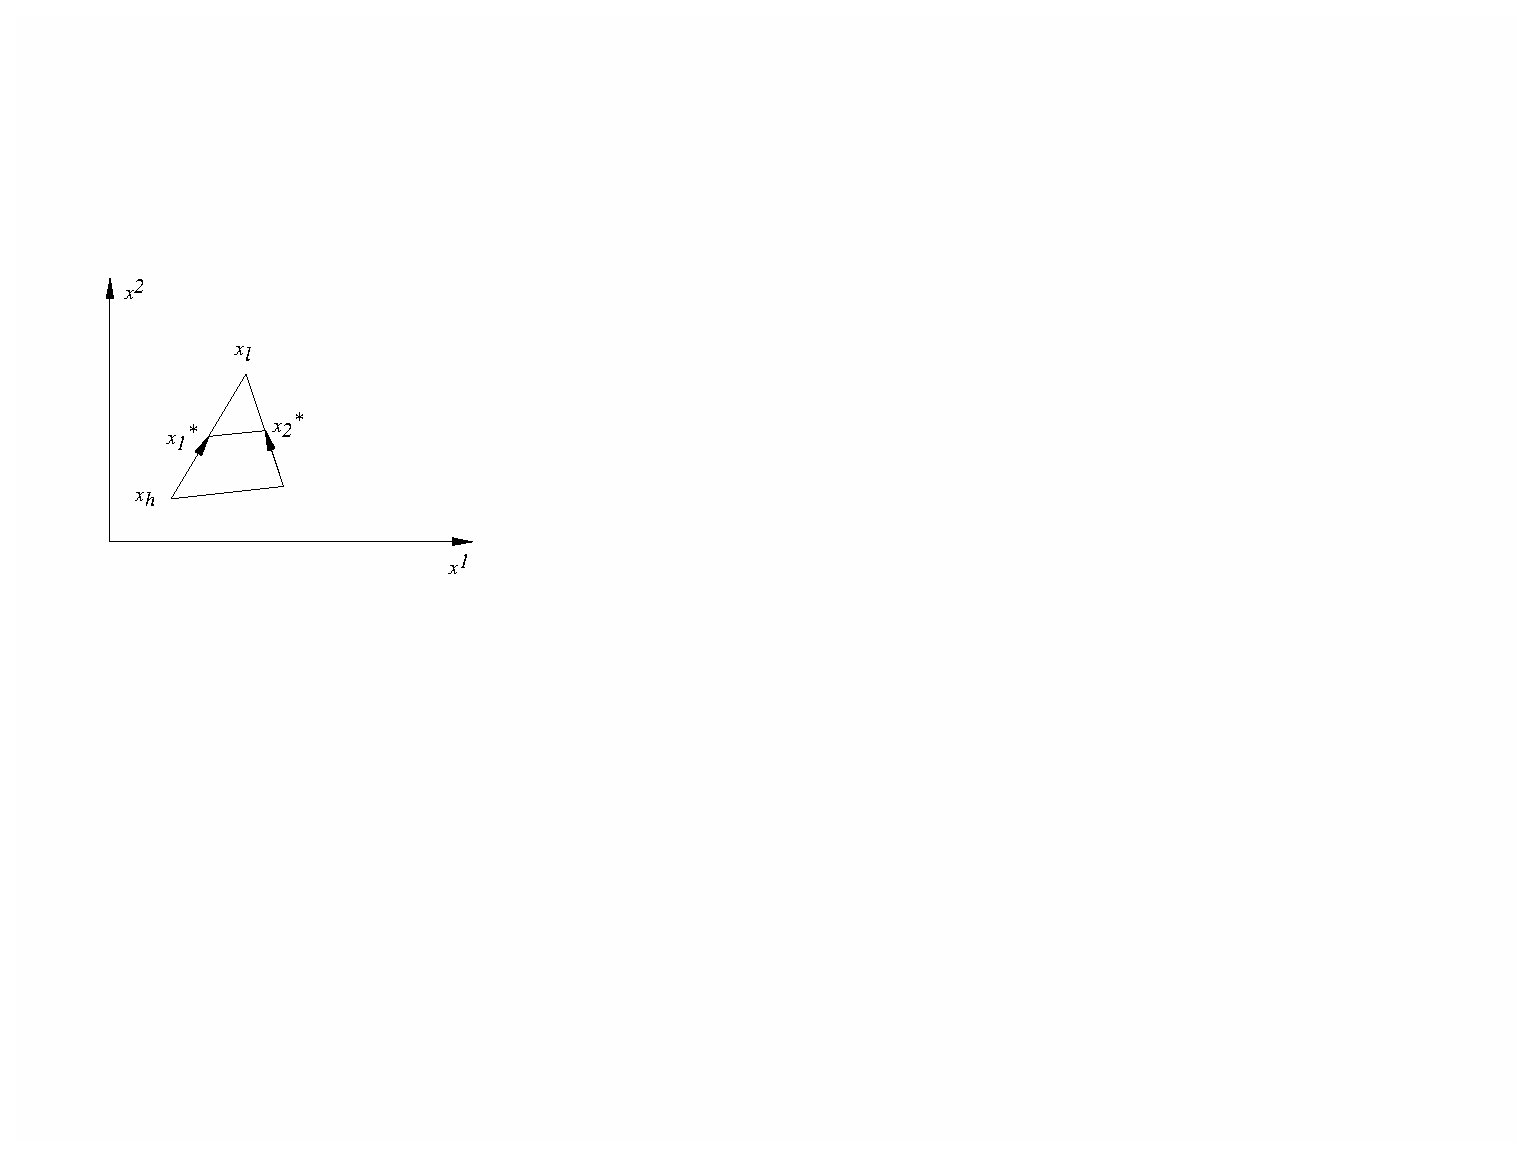
\epsfig
      {file=img/nel_mea_tot.eps, bb=35 265 225 420, scale=0.9, clip=}} }
  \caption{Simplex operations.}
  \label{fig:simOpeAll}
\end{figure}
The notation defined below is used in describing the main operations. The operations are illustrated in Fig.~\ref{fig:simOpeAll} where for simplicity 
a two-dimensional simplex is illustrated.\\

We now introduce some notation and definitions.
\begin{subequations}
\begin{enumerate}
\item We will denote by $\mathbf{I} \triangleq \{1, \, \ldots \, , \, n+1\}$
the set of all vertex indices.
\item
We will denote by $l \in \mathbf I$ the smallest index in $\mathbf I$
such that
\begin{equation}
l = \argmin_{i \in \mathbf{I} }  f(x_i).
\label{eq:simIndL}
\end{equation}
Hence, $f(x_l) \le f(x_i)$, for all $i \in \mathbf I$. 
\item
We will denote by $h \in \mathbf I$ the smallest index in $\mathbf I$
such that
\begin{equation}
h = \argmax_{i \in \mathbf{I} }  f(x_i).
\label{eq:simIndH}
\end{equation}
Hence, $f(x_h) \ge f(x_i)$, for all $i \in \mathbf I$. 
\item 
Let $x_i$, for $i \in \mathbf I$, denote the simplex vertices, and let $h$ be as in~\eqref{eq:simIndH}.
We will denote by $x_c \in \Re^n$ the {\em centroid} of the simplex, defined as
\begin{equation}
x_c \triangleq \frac{1}{n} \, 
\mathop{\sum_{i=1}}_{i \neq h}^{n+1} x_i
\label{eq:simCenDef}
\end{equation}
\end{enumerate}
\end{subequations}

Next, we introduce the three main operations.
\begin{subequations}
\begin{description}
\item[Reflection]
Let $h \in \mathbf I$ be as in~\eqref{eq:simIndH} and let
$x_c$ be as in~\eqref{eq:simCenDef}.
The reflection of $x_h \in \Re^n$ to a point denoted as 
$x^* \in \Re^n$ is defined as
\begin{equation}
   x^* \triangleq (1+\alpha) \, x_c - \alpha \, x_h,
\label{eq:simRefOpe}
\end{equation}
where $\alpha \in \Re$, with $\alpha > 0$, is
called the \emph{reflection coefficient}.

\item[Expansion of the simplex]
Let $x^* \in \Re^n$ be as in~\eqref{eq:simRefOpe} and
$x_c$ be as in~\eqref{eq:simCenDef}.
The expansion of $x^* \in \Re^n$ to a point denoted as 
$x^{**} \in \Re^n$ is defined as
\begin{equation}
   x^{**} \triangleq \gamma \, x^* + (1-\gamma) \, x_c,
\label{eq:simExp}
\end{equation}
where $\gamma \in \Re$, with $\gamma > 1$, is
called the \emph{expansion coefficient}.

\item[Contraction of the simplex]
Let $h \in \mathbf I$ be as in~\eqref{eq:simIndH} and
$x_c$ be as in~\eqref{eq:simCenDef}.
The contraction of $x_h \in \Re^n$ to a point denoted as 
$x^{**} \in \Re^n$ is defined as
\begin{equation}
   x^{**} \triangleq \beta \, x_h + (1 - \beta) \, x_c,
  \label{eq:simAlgCon}
\end{equation}
where $\beta \in \Re$, with $0 < \beta < 1$, is
called the \emph{contraction coefficient}.
\end{description}
\end{subequations}

% ---------------------------------
\subsection{Basic Algorithm}
In this section, we describe the basic Nelder and Mead algorithm~\cite{NelderMea1965}. 
The extension of O'Neill and the modified restart criterion are discussed later.
The algorithm is as follows:
\begin{enumerate}

\item Initialization: 
Given an initial iterate $x_1 \in \Re^n$,
a scalar $c$, with $c=1$ in the initialization,
a vector $s \in \Re^n$ with user-specified step sizes for each independent parameter,
and the set of unit coordinate vectors $\{ e_i \}_{i=1}^n$,
construct an initial simplex with vertices,
for $i \in \{1, \ldots , n \}$,
\begin{equation}
  x_{i+1} = x_1 + c \, s^i \, e_i.
\label{eq:simAlgIni}
\end{equation}
Compute $f(x_i)$, for $i \in \mathbf I$.
\item \label{des:simAlgRef} Reflection: 
Reflect the worst point, that is, compute $x^*$ as in~\eqref{eq:simRefOpe}.
\item \label{des:simAlgCheBes} Test whether we got the best point:
If $f(x^*) < f(x_l)$, expand the simplex using~\eqref{eq:simExp}
since further improvement in this direction is likely.
If $f(x^{**})< f(x_l)$, then 
$x_h$ is replaced by $x^{**}$,
otherwise $x_h$ is replaced by $x^*$, and 
the procedure is restarted from \ref{des:simAlgRef}.

\item 
If it turned out under \ref{des:simAlgCheBes} that $f(x^*) \ge f(x_l)$,
then we check if the new point $x^*$ is the worst of all points:
If $f(x^*) > f(x_i)$, for all $i \in \mathbf I$, with $i \ne h$, we contract 
the simplex (see \ref{des:simAlgCon}); 
otherwise we replace $x_h$ by $x^*$ and 
go to \ref{des:simAlgRef}.

\item \label{des:simAlgCon} 
For the contraction, we first check if we should try a partial outside 
contraction or a partial inside contraction: If $f(x^*) \ge f(x_h)$,
then we try a partial inside contraction.
To do so, we leave our indices as is and 
apply (\ref{eq:simAlgCon}). 
Otherwise, we try a partial outside contraction. 
This is done 
by replacing $x_h$ by $x^*$ and applying (\ref{eq:simAlgCon}). 
After the partial inside or the partial outside contraction,
we continue at \ref{des:simAlgCheWor}.

\item \label{des:simAlgCheWor}
If $f(x^{**}) \ge f(x_h)$\footnote{ Nelder and Mead~\cite{NelderMea1965} use the strict 
inequality $f(x^{**}) > f(x_h)$.
However, if the user writes the cost function value with only a few 
representative digits to a text file, 
then the function looks like a step function if slow convergence is 
achieved. In such cases, $f(x^{**})$ might sometimes be equal to $f(x_h)$.
Experimentally, it has been shown 
advantageous to perform a total contraction rather than continuing with a reflection. 
Therefore, the strict inequality has been changed to a weak inequality.},
we do a total contraction of the 
simplex by replacing $x_i \leftarrow (x_i + x_l)/2$, for all $i \in \mathbf I$.
Otherwise, we replace $x_h$ by $x^{**}$. 
In both cases, we continue from \ref{des:simAlgRef}.
\end{enumerate}

\begin{figure}
\centering
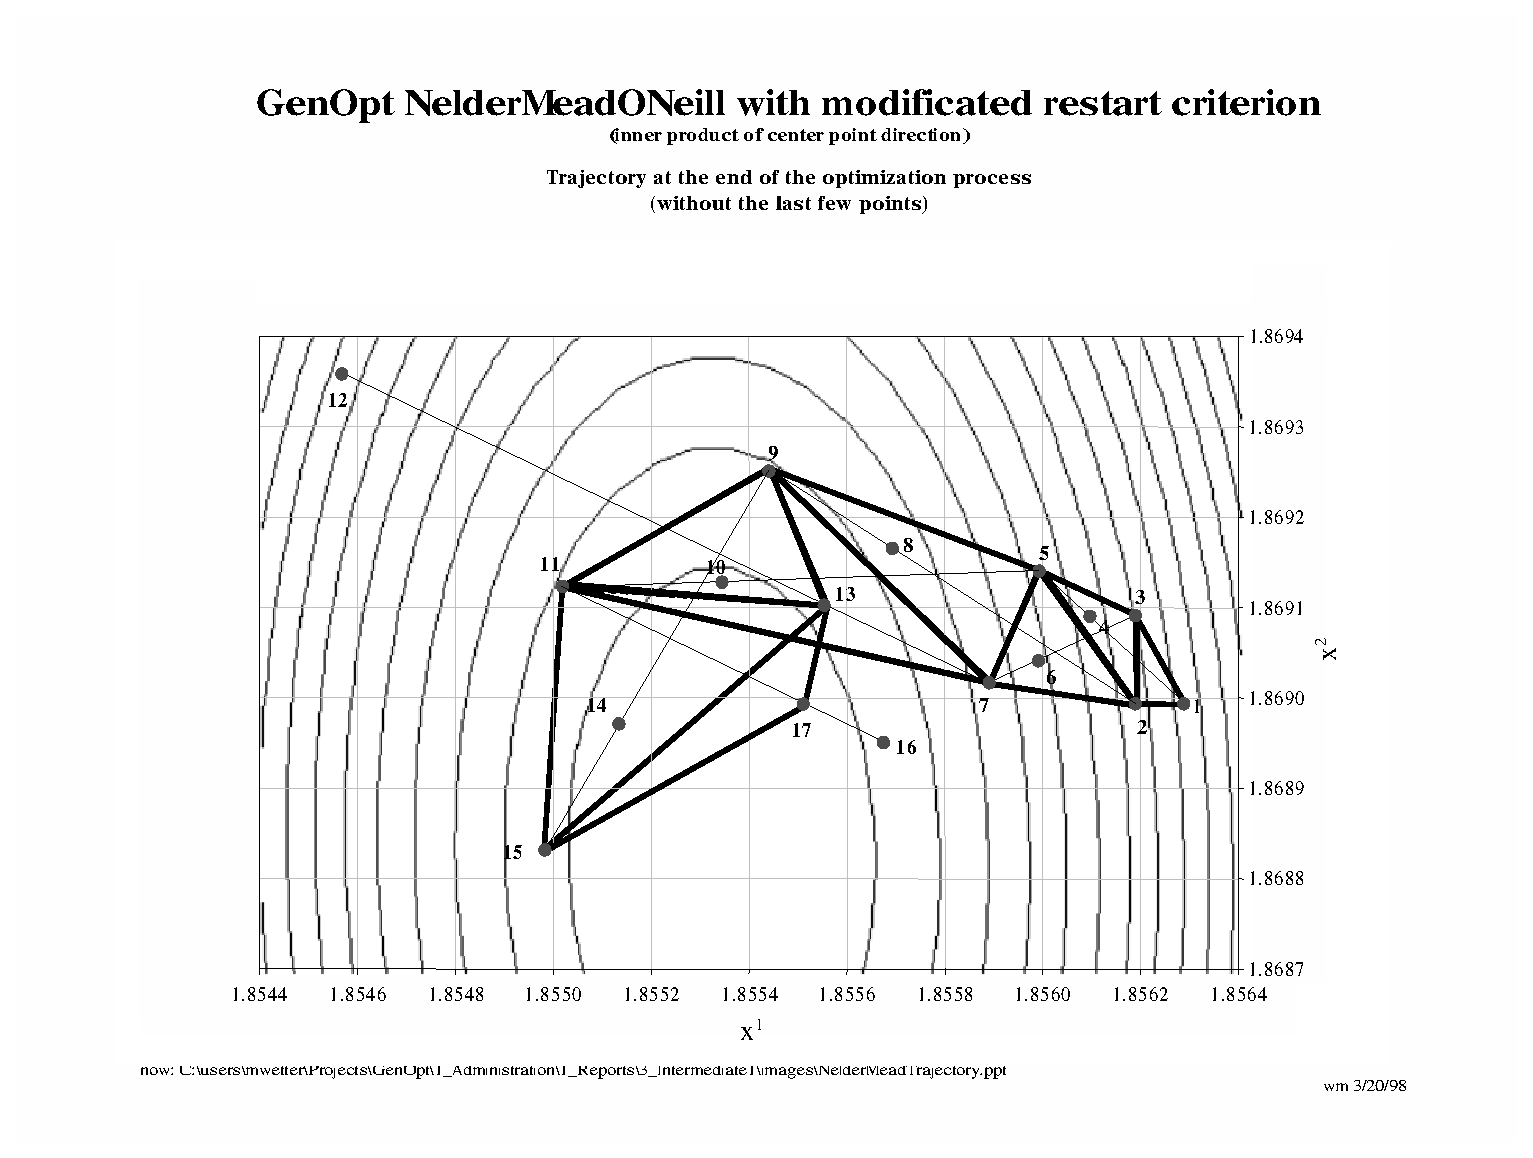
\epsfig{file=img/nel_mea_mov_tra.eps, bb=98 47 640 400, width=\headwidth, clip=}
\caption{Sequence of iterates generated by the Simplex algorithm.}
\label{fig:simSeqAlg}
\end{figure}



Fig. \ref{fig:simSeqAlg} shows a contour plot of a cost function $f \colon \Re^n \to \Re$ with a sequence of iterates
generated by the Simplex algorithm.
The sequence starts with 
constructing an initial simplex $x_1$, $x_2$, $x_3$. $x_1$ has the highest function value and is therefore 
reflected, which generates $x_4$. $x_4$ is the best point in the set $\{x_1, x_2, x_3, x_4\}$. Thus, it is further 
expanded, which generates $x_5$. $x_2$, $x_3$ and $x_5$ now span the new simplex. In this simplex, $x_3$ is the 
vertex with the highest function value and hence goes over to $x_6$ and further to $x_7$. The process of reflection 
and expansion is continued again two times, which leads to the simplex spanned by $x_7$, $x_9$ and 
$x_{11}$. $x_7$ goes over to $x_{12}$ which turns out to be the worst point. Hence, we do a partial inside 
contraction, which generates $x_{13}$. $x_{13}$ is better than $x_7$ so we use the simplex spanned by $x_9$, 
$x_{11}$ and $x_{13}$ for the next reflection. 
The last steps of the optimization are for clarity not shown.


% ---------------------------------

\subsection{Stopping Criteria}
The first criterion is a test of the variance of the function values at the vertices of the simplex
\begin{equation}
\frac{1}{n} \, \left(
\sum_{i=1}^{n+1} \bigl( f(x_i) \bigr)^2 -
   \frac{1}{n+1} \, \left(\sum_{i=1}^{n+1} f(x_i)    \right)^2 \, 
\right) < \epsilon^2,
 \label{eq:neaMeaVar}
\end{equation}
then the original implementation of the algorithm stops.
Nelder and Mead have chosen this stopping criterion based on the statistical problem
of finding the minimum of a sum of squares surface.
In this problem, the curvature near the minimum yields information about
the unknown parameters.
A slight curvature indicates a high sampling variance of the estimate.
Nelder and Mead argue that in such cases, there is no reason for finding 
the minimum point with high accuracy.
However, if the curvature is marked, 
then the sampling variance is low and a higher accuracy in determining the optimal parameter set is desirable.

Note that the stopping criterion~\eqref{eq:neaMeaVar} requires the variance
of the function values at the simplex vertices to be smaller 
than a prescribed limit.
However, if $f(\cdot)$ has large discontinuities, which has been observed
in building energy optimization problems~\cite{WetterWright2003:1},
then the test~\eqref{eq:neaMeaVar} may never be satisfied.
For this reason, among others, 
we do not recommend using this algorithm if the cost function
has large discontinuities.

\pagebreak[4]
% -------------------
\subsection{O'Neill's Modification}
O'Neill modified the termination criterion by adding a further condition~\cite{ONeill1971}. He checks 
whether any orthogonal step, each starting from the best vertex of the current simplex, leads to a further 
improvement of the cost function. 
He therefore sets $c = 0.001$ and tests if
\begin{subequations}
\label{eq:optCheNelMeaOri}
\begin{equation}
  f(x_l) < f(x)
\label{eq:optCheNelMeaOriCon}
\end{equation}
for all $x$ defined by
\begin{equation}
   x \triangleq x_l + c \, s^i \, e_i, \qquad i \in \{1, \ldots , n \},
  \label{eq:optCheNelMeaOriCoo}
\end{equation}
where $x_l$ denotes the best known point,
and $s^i$ and $e_i$ are as in \eqref{eq:simAlgIni}.\\

% ----------------------------
\subsection{Modification of Stopping Criteria}

In GenOpt, (\ref{eq:optCheNelMeaOri}) has been modified. It has been observed that users sometimes 
write the cost function value with only few representative digits to the output file. 
In such cases, 
(\ref{eq:optCheNelMeaOriCon}) is not satisfied if the write statement 
in the simulation program truncates 
digits so that the difference $f(x_l)-f(x)$, where $f\depd$ denotes the value that is
read from the simulation output file, is zero.
To overcome this numerical problem, 
(\ref{eq:optCheNelMeaOriCoo}) has been modified to
\begin{equation}
   x = x_l + \exp(j) \, c \, s^i \, e_i, \qquad i \in \{1, \ldots , n \}
\label{eq:optCheNelMeaOriMod}
\end{equation}
\end{subequations}
where for each direction $i \in \{1, \ldots , n \}$, 
the counter $j \in \Na$ is set to zero for the first trial and increased by one as long as 
$f(x_l) = f(x)$.

If (\ref{eq:optCheNelMeaOriCon}) fails for any direction, then $x$ computed by 
(\ref{eq:optCheNelMeaOriMod}) is the new starting point and a new simplex with side lengths $(c\, s^i)$, $i \in \{1, \ldots, n\}$, is constructed.
The point $x$ that failed (\ref{eq:optCheNelMeaOriCon}) is then used as the initial point $x_l$ in (\ref{eq:simAlgIni}).\\


\begin{figure}
  \mbox{ \subfigure[Sequence of iterates in the neighborhood of the minimum.]{
  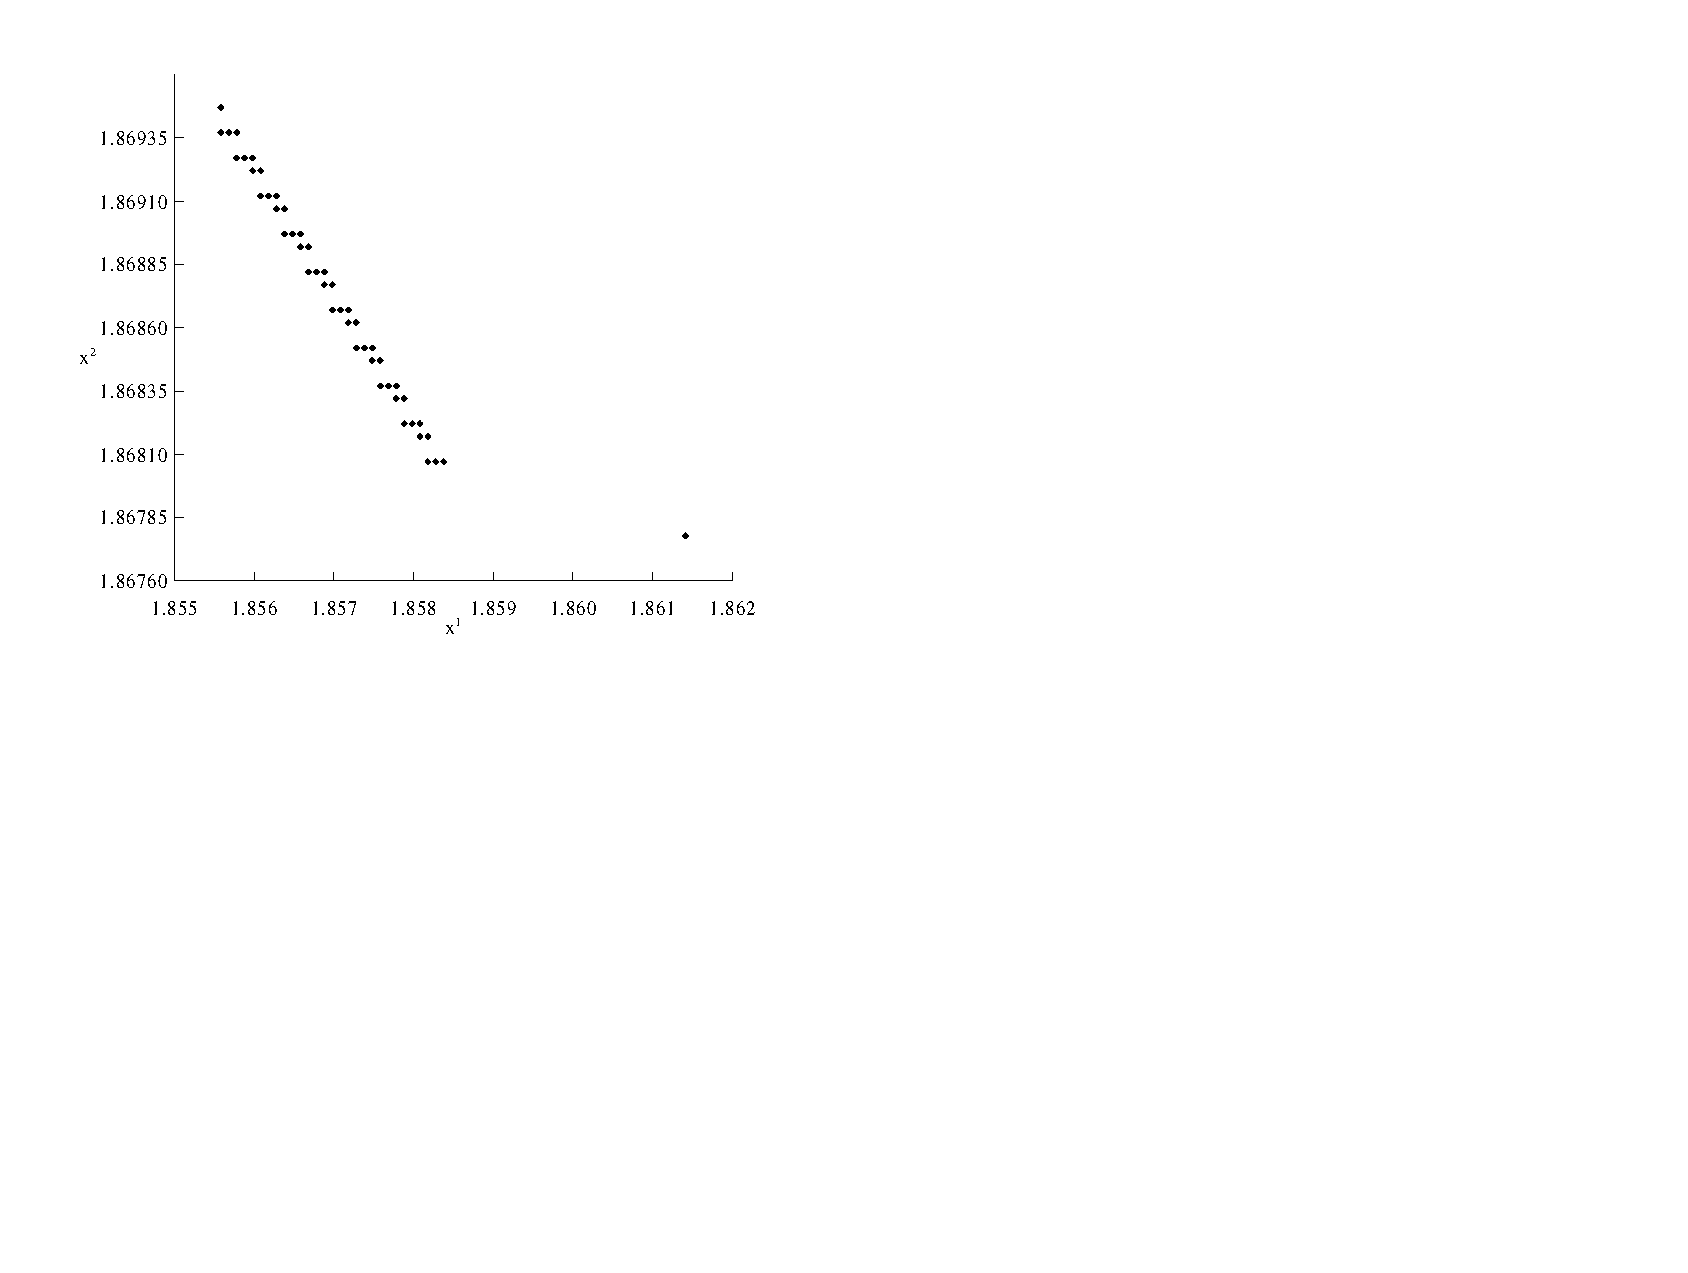
\epsfig{file=img/nel_mea_res_tra.eps, bb=25 290 360 575, clip=, width=0.5\headwidth} \label{fig:neaMeaResTra} } \quad
\subfigure[2-dimensional test function ``2D1''.]{
  \epsfig{file=img/fun_f2d1.eps, bb=120 95 740 500, width=0.5\headwidth} 
\label{fig:neaMeaTesFun} } }
\caption{Nelder Mead trajectory.}
\end{figure}
Numerical experiments showed that during slow convergence the algorithm was restarted too frequently.

Fig.~\ref{fig:neaMeaResTra} shows a sequence of iterates where the algorithm was restarted too frequently.
The iterates in the figure are part of the iteration sequence near the
minimum of the test function shown in Fig.~\ref{fig:neaMeaTesFun}. 
The algorithm gets close to the minimum with appropriately large steps.
The last of these steps can be seen at the right of the figure.
After this step, the stopping criterion (\ref{eq:neaMeaVar}) was satisfied 
which led to a restart check, followed by a new construction of the simplex. From there on, the 
convergence was very slow due to the small step size. After each step, the stopping criterion was satisfied 
again which led to a new test of the optimality condition (\ref{eq:optCheNelMeaOriCon}), followed by a 
reconstruction of the simplex. This check is very costly in terms of function evaluations and, furthermore, 
the restart with a new simplex does not allow increasing the step size, though we are heading locally in 
the right direction.\\

O'Neill's modification prevents both excessive checking of the optimality condition as well as excessive 
reconstruction of the initial simplex. This is done by checking for convergence only after a predetermined 
number of steps (e.g., after five iterations). 
However, the performance of the algorithm depends 
strongly on this number. As an extreme case, a few test runs were done where convergence was checked 
after each step as in Fig. \ref{fig:neaMeaResTra}. It turned out that in some cases no convergence was 
reached within a moderate number of function evaluations if $\epsilon$ in (\ref{eq:neaMeaVar}) is chosen 
too large, e.g., $\epsilon = 10^{-3}$ (see Tab. \ref{tab:nelMeaBenMarRes}).\\

\pagebreak[2]
To make the algorithm more robust, it is modified based on the following arguments:
\begin{enumerate}
\item
If the simplex is moving in the same direction in the last two steps, then the search is not 
interrupted by checking for optimality since we are making steady progress in the moving direction.
\item
If we do \emph{not} have a partial inside or total contraction immediately beyond us, then it is likely 
that the minimum lies in the direction currently being explored. 
Hence, we do not interrupt the search with a restart.
\end{enumerate}

These considerations have led to two criteria that both have to be satisfied to permit the convergence check according to (\ref{eq:neaMeaVar}), which might be followed by a check for optimality.\\

First, it is checked if we have done a partial inside contraction or a total contraction. If so, we 
check if the direction of the latest two steps in which the simplex is moving has changed by an angle of at 
least $(\pi / 2)$. 
To do so, we introduce the center of the simplex, defined by
\begin{equation}
  x_m \triangleq \frac{1}{n+1} \, \sum_{i=1}^{n+1} x_i,
\end{equation}
where $x_i$, $i \in \{ 1, \ldots, n\}$, are the simplex vertices.
We also introduce the normalized direction of the simplex between two steps,
\begin{equation}
  d_k \triangleq \frac{ x_{m, k} - x_{m, k-1} }
{ \| x_{m, k} - x_{m, k-1} \| },
\end{equation}
where $k \in \Na$ is the current iteration number.

We determine how much the simplex has changed its direction $d_k$ between two steps by 
computing the inner product $\langle d_{k-1}, d_k \rangle$. 
The inner product is equal to the cosine of the angle $d_{k-1}$ and $d_k$.
If
\begin{equation}
  \cos \phi_k = \langle d_{k-1}, \, d_k \rangle \le 0,
  \label{eq:nelMeaCosMov}
\end{equation}
then the moving direction of the simplex has changed by at least $\pi / 2$.
Hence, the simplex has changed the exploration direction.
Therefore, a minimum might be achieved and we need to test the variance of the 
vertices (\ref{eq:neaMeaVar}), possibly followed by a test of (\ref{eq:optCheNelMeaOriCon}).\\

%---
Besides the above modification, a further modification was tested: 
In some cases, a reconstruction of the simplex after a failed check (\ref{eq:optCheNelMeaOriCon})
yields to slow convergence.
Therefore, the algorithm was modified so that it continues at 
point \ref{des:simAlgRef} on page~\pageref{des:simAlgRef} without reconstructing the simplex after 
failing the test (\ref{eq:optCheNelMeaOriCon}).
However, reconstructing the simplex led in most of the benchmark tests to faster convergence. Therefore, 
this modification is no longer used in the algorithm.

\subsection{Benchmark Tests}
\label{sec:algSimBenTes}

\begin{table}
\newcolumntype{C}{>{\centering\arraybackslash}X}
\begin{tabularx}{\headwidth}{|p{2cm}|C|C|C|C|C|C|C|C|}
\hline
 & \multicolumn{8}{|c|}{Accuracy} \\ \cline{2-9}
& \multicolumn{4}{|c|}{$\epsilon = 10^{-3}$} & \multicolumn{4}{|c|}{$\epsilon = 10^{-5}$} \\ \hline
\raggedright Test function & Rosen-brock & 2D1 & Quad with I matrix & Quad with Q matrix & Rosen-brock & 2D1 & Quad with I matrix & Quad with Q matrix \\ \hline
\raggedright Original, with reconstruction &  137  &  120  &  3061  &  1075  &  139  &  109  &  1066  &  1165 \\ \hline
\raggedright Original, no reconstruction &  136  &  110  &  1436  &  1356  &  139  &  109  &  1433  &  1253 \\ \hline
\raggedright Modified, with reconstruction &  145  &  112  &  1296  &  1015  &  152  &  111  &  1060  &  1185 \\ \hline
\raggedright Modified, no reconstruction &  155  &  120  &  1371  &  1347  &  152  &  109  &  1359  &  1312 \\ \hline
\end{tabularx}
\caption{Comparison of the number of function evaluations for different implementations of the simplex algorithm. See Appendix for the definition of the function.}
\label{tab:nelMeaBenMarRes}
\end{table}

\begin{figure}
  \centering
  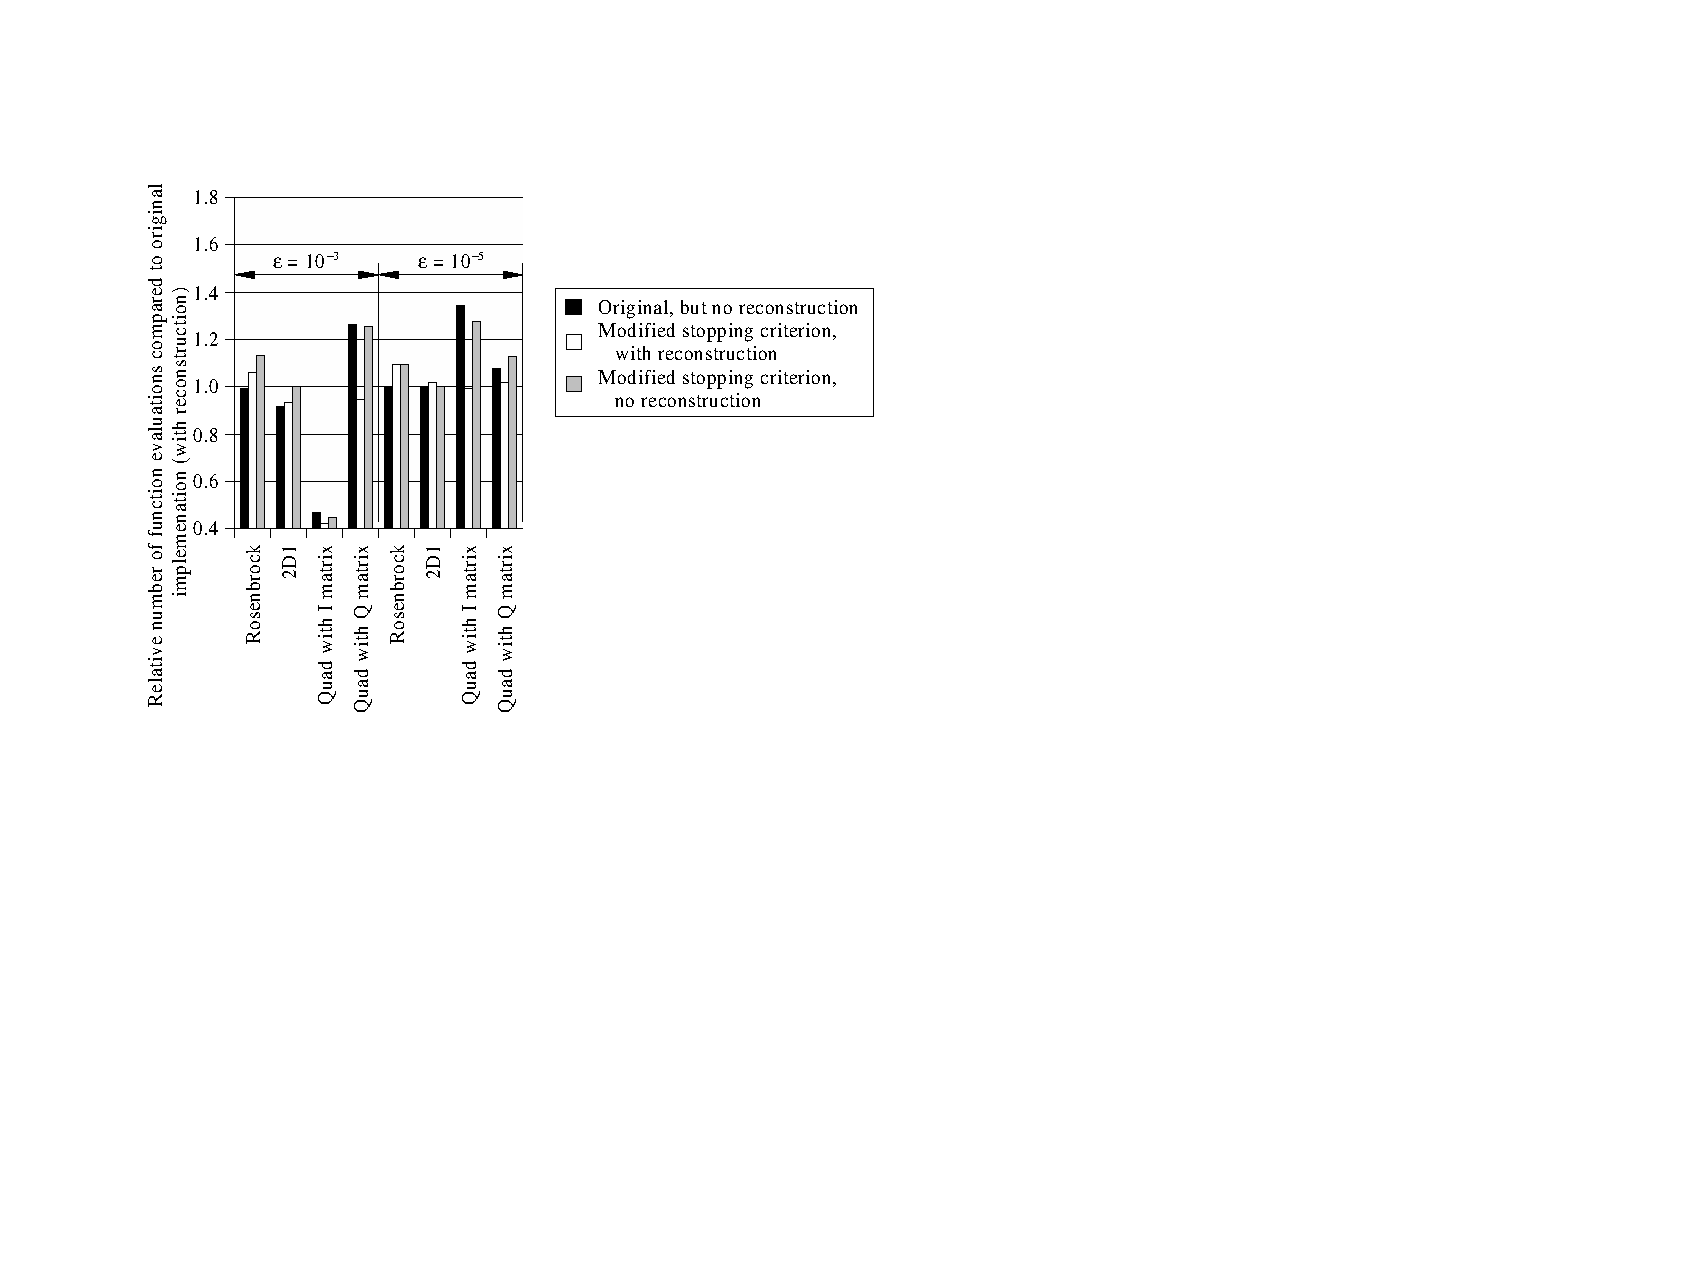
\epsfig{file=img/nel_mea_ben.eps, bb=60 255 420 520, clip=} 
  \caption{Comparison of the benchmark tests.}
  \label{fig:nelMeaBenMarRes}
\end{figure}

Tab.~\ref{tab:nelMeaBenMarRes} shows the number of function evaluations and 
Fig.~\ref{fig:nelMeaBenMarRes} shows the relative number of function evaluations compared to the original 
implementation for several test cases. The different functions and the parameter settings are given in the 
Appendix. 
The only numerical parameter that was changed for the different optimizations is the accuracy, $\epsilon$.\\

It turned out that modifying the stopping criterion is effective in most cases, 
particularly if a new simplex is constructed after the check~\eqref{eq:optCheNelMeaOriCon} failed.
Therefore, the following two versions of the simplex algorithm are implemented in GenOpt:
\begin{enumerate}
\item
The base algorithm of Nelder and Mead, including the extension of O'Neill.
After failing~\eqref{eq:optCheNelMeaOriCon},
the simplex is \emph{always} reconstructed with the new step size.
\item 
The base algorithm of Nelder and Mead, including the extension of O'Neill,
but with the modified stopping criterion as explained above.
That is, the simplex is only reconstructed if its moving direction changed, 
and if we have an inside or total construction beyond us.
\end{enumerate}

\subsection{Keywords}
For the Simplex algorithm, the command file (see page~\pageref{par:comFil}) must only contain continuous parameters.\\

To invoke the Simplex algorithm, the \texttt{Algorithm} section of the GenOpt command file must 
have following form:
\begin{lstlisting}
Algorithm{
   Main                    = NelderMeadONeill;
   Accuracy                = Double;   // 0 <  Accuracy
   StepSizeFactor          = Double;   // 0 <  StepSizeFactor
   BlockRestartCheck       = Integer;  // 0 <= BlockRestartCheck
   ModifyStoppingCriterion = Boolean;
}
\end{lstlisting}

\noindent The key words have following meaning:
\begin{codedescription}
\item[Main]
   The name of the main algorithm.
\item[Accuracy]
The accuracy that has to be reached before the optimality condition is checked. \texttt{Accuracy} is 
defined as equal to $\epsilon$ of (\ref{eq:neaMeaVar}), page~\pageref{eq:neaMeaVar}.

\item[StepSizeFactor]
A factor that multiplies the step size of each parameter for 
(a) testing the optimality condition and 
(b) reconstructing the simplex.
\texttt{StepSizeFactor} is equal to $c$ in 
(\ref{eq:simAlgIni}) and (\ref{eq:optCheNelMeaOriMod}).

\item[BlockRestartCheck]
Number that indicates for how many main iterations the restart criterion is not checked. If zero, restart 
might be checked after each main iteration.

\item[ModifyStoppingCriterion]
Flag indicating whether the stopping criterion should be modified. 
If \texttt{true}, then the optimality check 
(\ref{eq:neaMeaVar}) is done only if both of the following conditions are satisfied: 
(a) in the last step, either a partial inside contraction or total contraction was done, and 
(b) the moving direction of the simplex has changed by an angle $\phi_k$ of at least $(\pi/2)$, 
where $\phi_k$ is computed using (\ref{eq:nelMeaCosMov}).
\end{codedescription}


